
%%%%%%%%%%%%%%%%%%%%%%%%%%%%%%%%%%%%%%%%%%%%%%%%%%%%%%%%%%%%%%%%%%%%%%%%%%%%%%%%%%%%%%%
%%%%%%%%%%%%%%%%%%%%%%%%%%%%%%%%%%%%%%%%%%%%%%%%%%%%%%%%%%%%%%%%%%%%%%%%%%%%%%%%%%%%%%%
% 
% This top part of the document is called the 'preamble'.  Modify it with caution!
%
% The real document starts below where it says 'The main document starts here'.

\documentclass[12pt]{article}

\usepackage{amssymb,amsmath,amsthm}
\usepackage[top=1in, bottom=1in, left=1.25in, right=1.25in]{geometry}
\usepackage{fancyhdr}
\usepackage{enumerate}
\usepackage{listings}
\usepackage{graphicx}
\usepackage{float}

% Comment the following line to use TeX's default font of Computer Modern.
\usepackage{times,txfonts}



\makeatletter
\renewcommand*\env@matrix[1][*\c@MaxMatrixCols c]{%
  \hskip -\arraycolsep
  \let\@ifnextchar\new@ifnextchar
  \array{#1}}
\makeatother

\newtheoremstyle{homework}% name of the style to be used
  {18pt}% measure of space to leave above the theorem. E.g.: 3pt
  {12pt}% measure of space to leave below the theorem. E.g.: 3pt
  {}% name of font to use in the body of the theorem
  {}% measure of space to indent
  {\bfseries}% name of head font
  {:}% punctuation between head and body
  {2ex}% space after theorem head; " " = normal interword space
  {}% Manually specify head
\theoremstyle{homework} 

% Set up an Exercise environment and a Solution label.
\newtheorem*{exercisecore}{Exercise \@currentlabel}
\newenvironment{exercise}[1]
{\def\@currentlabel{#1}\exercisecore}
{\endexercisecore}

\newcommand{\localhead}[1]{\par\smallskip\noindent\textbf{#1}\nobreak\\}%
\newcommand\solution{\localhead{Solution:}}

%%%%%%%%%%%%%%%%%%%%%%%%%%%%%%%%%%%%%%%%%%%%%%%%%%%%%%%%%%%%%%%%%%%%%%%%
%
% Stuff for getting the name/document date/title across the header
\makeatletter
\RequirePackage{fancyhdr}
\pagestyle{fancy}
\fancyfoot[C]{\ifnum \value{page} > 1\relax\thepage\fi}
\fancyhead[L]{\ifx\@doclabel\@empty\else\@doclabel\fi}
\fancyhead[C]{\ifx\@docdate\@empty\else\@docdate\fi}
\fancyhead[R]{\ifx\@docauthor\@empty\else\@docauthor\fi}
\headheight 15pt

\def\doclabel#1{\gdef\@doclabel{#1}}
\doclabel{Use {\tt\textbackslash doclabel\{MY LABEL\}}.}
\def\docdate#1{\gdef\@docdate{#1}}
\docdate{Use {\tt\textbackslash docdate\{MY DATE\}}.}
\def\docauthor#1{\gdef\@docauthor{#1}}
\docauthor{Use {\tt\textbackslash docauthor\{MY NAME\}}.}
\makeatother

% Shortcuts for blackboard bold number sets (reals, integers, etc.)
\newcommand{\Reals}{\ensuremath{\mathbb R}}
\newcommand{\Nats}{\ensuremath{\mathbb N}}
\newcommand{\Ints}{\ensuremath{\mathbb Z}}
\newcommand{\Rats}{\ensuremath{\mathbb Q}}
\newcommand{\Cplx}{\ensuremath{\mathbb C}}
%% Some equivalents that some people may prefer.
\let\RR\Reals
\let\NN\Nats
\let\II\Ints
\let\CC\Cplx

%%%%%%%%%%%%%%%%%%%%%%%%%%%%%%%%%%%%%%%%%%%%%%%%%%%%%%%%%%%%%%%%%%%%%%%%%%%%%%%%%%%%%%%
%%%%%%%%%%%%%%%%%%%%%%%%%%%%%%%%%%%%%%%%%%%%%%%%%%%%%%%%%%%%%%%%%%%%%%%%%%%%%%%%%%%%%%%
% 
% The main document start here.

% The following commands set up the material that appears in the header.
\doclabel{STAT 401: Homework 2}
\docauthor{Stefano Fochesatto}
\docdate{\today}

\begin{document}

\begin{exercise}{1.5} Can southern california's water supply in future years be predicted
    from past data? One factor affecting water availability is stream 
    runoff. If runoff could be predicted
    engineers, planners, and policy makers could do their jobs more efficiently. 
    The data file contains 43 years work of precipitation measurements taken at six sites in Sierra Nevada mountains
    and stream runoff volume at a site near Bishop, California. Draw a scatter plot for these data and 
    summarize the information from these plots. \\
    \solution Loading in our data and creating a scatter plot matrix we get the following visualization, 
        \begin{figure}[H]
            \begin{center}
            \caption{Correlation Scatter Matrix for SRV}
            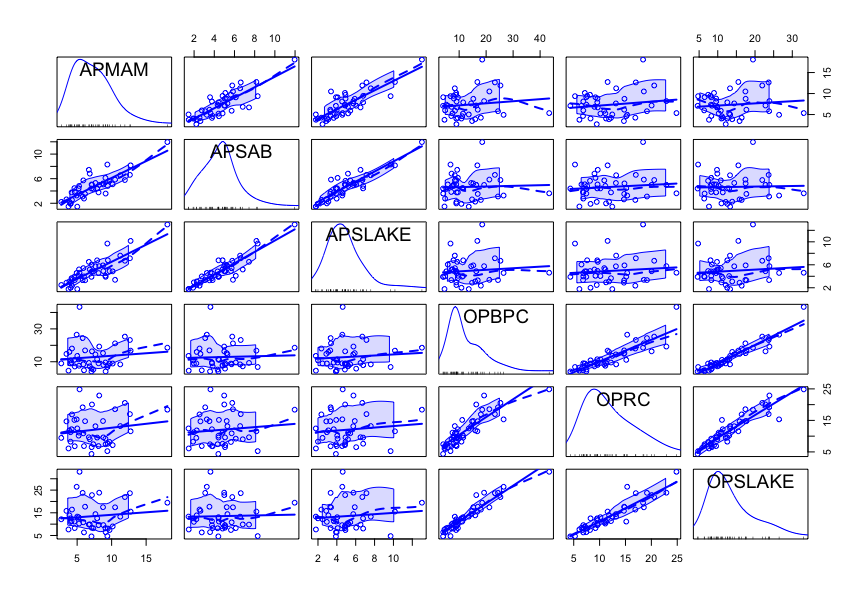
\includegraphics[ width= \textwidth]{Rplot.png}
            \end{center}
        \end{figure}
    We can see that there is a strong positive correlation between the OPSLAKE, OPRC, and OPBC sites. 
    There is also a strong positive correlation between the APSLAKE, APSAB, and APMAM sites. The rest of the 
    scatter plots exhibit high variance and little to no correlation. This is likely due to the fact that stream runoff was 
    measured in 2 places, the Sierra Nevada Mountains, and Bishop, California. All plots seem to be positively skewed 
    from the presence of an outlier. Looking into the data it seems like 1962 was a strong year for runoff in Bishop, California
    and 1982 was a strong year in the Sierra Nevada Mountains. 
\end{exercise}
\textbf{Code:}
\begin{center}
    \lstinputlisting{r1.txt}
\end{center}
\newpage


\begin{exercise}{2} For the data set in problem 1.5, do the following
    \begin{enumerate}
        \item Give at least two possible ways in which the data set could be inadequate 
        for building a useful prediction model for stream runoff near Bishop, California. \\
        \solution While data from all sites looks to have a close constant variance its clear that in 
        general the variance is relatively very high and we would be hard pressed to create a predictive linear model
        that is accurate. \\

        In general all the data is positively skewed with the OPBC and OPSLAKE sites in particular having very high outliers.
        Not addressing these extreme values can cause a linear model to be less accurate. 
        \textbf{Code:}
            \begin{center}
                     \lstinputlisting{r2.txt}
            \end{center}
        \vspace{.25in}
        \item Does the data set result form an observational, or experimental, study?\\
        
        \solution Since the researchers weren't purposefully manipulating some variable in an effort to 
        measure a response, this data is observational data. The goal is to collect data without interfering. 
        \vspace{.25in}

        \item Give at least three important questions that a person might have about the data
        set before performing inferential analysis on it.\\
        \solution Primarily we want to know the Sampling Method used to recover the data. This will influence how we 
        estimate the parameters we want to know. We also want to now how dirty or clean the data is, if there were issues or changes
        in how the data was recovered, those things need to be taken into account during our analysis. We also want to have some idea of 
        how the data is distributed(Can we assume normality?)
        \vspace{.25in}

        \item Create some kind of plot or visualization to answer one of the questions you listed in the last part.\\
        \solution The following is a histogram of the runoff volume in the OPSLAKE site. This gives us an idea of the 
        how the data is distributed. It seems like it might be normal with a slight positive skew because of the outlier value. 
        We might benefit from bootstrapping this data. \\
        \begin{figure}[H]
            \begin{center}
            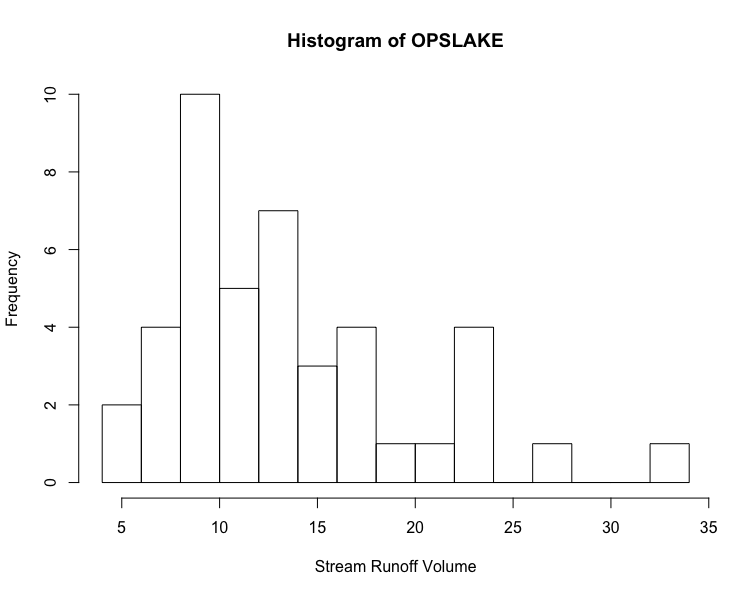
\includegraphics[ width= \textwidth]{Rplot2.png}
            \end{center}
        \end{figure}
        \textbf{Code:}
            \begin{center}
            \lstinputlisting{r3.txt}
            \end{center}
\newpage
    \end{enumerate}
\end{exercise}
\newpage

\begin{exercise}{1.4} The data file gives information about eruptions of Old Faithful Geyser 
    during October 1980. variables are the $Duration$ in seconds of the current eruptions, and the $Interval$, 
    the time in minutes to the next eruption, The data were collected by volunteers and were provided by the late 
    Roderick Hutchinson. Apart form missing data for the period from midnight to 6 a.m. This is a complete 
    record of eruptions for that month. Draw the relevant summary graph for predicting interval from duration and 
    summarize your results. \\
    \solution Importing the data and plotting with r, we get the following scatterplot, 
    \begin{figure}[H]
        \begin{center}
        \caption{Duration vs. Interval ScatterPlot}
        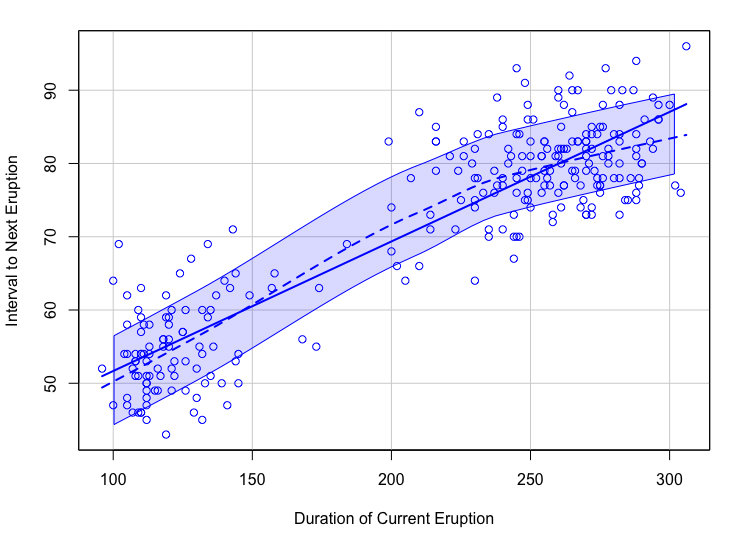
\includegraphics[ width= \textwidth]{Rplot3.png}
        \end{center}
    \end{figure}
    Looking at the scatter plot, beyond the positive correlation between duration and interval the data appears to be bimodal. There seems to be a point where if 
    the duration is around 200 seconds or more the interval to the next eruption is greater than 70
    while if the duration is less than 200 the interval for the next eruption is less than 70.  
\end{exercise}
\newpage

\begin{exercise}{4} For the data set in problem 1.4 do the following, 
    \begin{enumerate}
        \item Identify the predictor and response.\\

        \solution In this data set we use the duration is the predictor variable and 
        the interval is the response variable. 
        \vspace{.25in}
        \item Does the data enable you to make claims about causation, or merely association?\\
        \solution This is another example of data that is observational, since we had no role in 
        changing the duration variable, or even developing a control duration variable. As a result we can 
        only make claims about association. 
        \vspace{.25in}
        \item Does the straight-line mean function seems to be plausible for this data set? Why or why not?
        \solution For the most part the variability seems to be constant, I would be worried around the 200 seconds interval
        but I think more data would need to be collected to say for sure.
        \vspace{.25in}
        \item Give the mean function and variance function (in terms of $\beta_0, \beta_1$ and $\sigma^2$) that would 
        comprise a linear model for this data set. 
        \solution Using the lm function in r we get that, 
        \begin{equation*}
            E(Interval|Duration = x) = B_0 + B_1x = 33.988 + .177x 
        \end{equation*}
        \begin{equation*}
            Var(Interval|Duration = x)= \sigma^2 = (1.182)^2
        \end{equation*}

        \textbf{Code:}
            \begin{center}
            \lstinputlisting{r4.txt}
            \end{center}
    \end{enumerate}
\end{exercise}
\newpage

\begin{exercise}{1.6} Provide a brief description between the five ratings described in the data 
    from ratemyprofessor.com. 
    \begin{figure}[H]
        \begin{center}
        \caption{Average professor ratings from ratemyprofessor.com}
        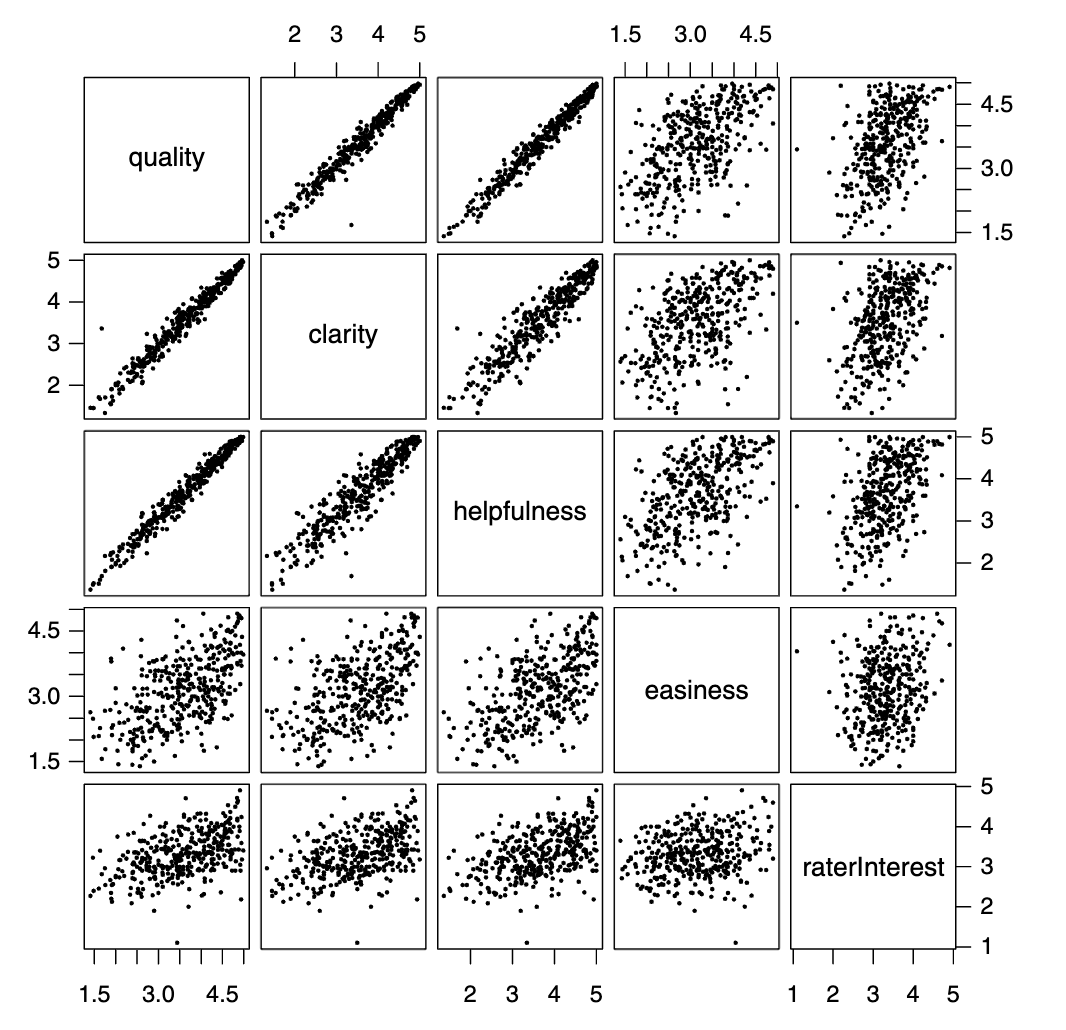
\includegraphics[ width= \textwidth]{plot1.png}
        \end{center}
    \end{figure}
    \solution From the plot we can see that there is a strong positive correlation between 
    the quality, clarity and helpfulness of the professor ratings. Furthermore it seems like easiness and 
    raterinterest are relatively uncorrelated with the rest of the data which might suggest that in aggregate the ratings are unbiased. 
    
\end{exercise}




\end{document}





















